\documentclass[12pt, a4paper]{article}

\usepackage[utf8]{inputenc}
\usepackage{graphicx}
\usepackage{float}

\graphicspath{{../diagrams/images/}{../diagrams/images/png/}}

\title{Progetto Ingegneria del Software}
\author{Davide Bleggi \and Joshua Chapman}
\date{Giugno 2020}


\begin{document}
\begin{titlepage}
  \maketitle
\end{titlepage}

\begin{abstract}
  Progetto per la creazione di un sistema informatico per gestire il servizio 
  di spesa on-line di un supermercato.
\end{abstract}

% Table of content
\tableofcontents
\newpage


\section{Introduzione}
% Subsection divisione del lavoro, tentativo di scrum, e difficoltà della distanza
% Paired developement
Date le distanze, i tempi ristretti, e il nostro team composto da sole due persone abbiamo preferito usare al \textbf{XP programming}, in grado di adattarsi meglio alle nostre esigenze, e appoggiandoci ad un servizio di \textbf{Version Control System} quale \textbf{GIT} per poter proseguire anche in autonomia e non solo con l'ausilio del \textbf{pair programming}. Quindi durante la progettazione è stato tenuto un approccio \textbf{Test First Developement} seguito da costanti aggiornamenti di \textbf{refactoring}.

\subsection{Analisi Dei Requisiti}
% Cominciato con analisi dei requisiti, sezioni del pdf
% Backlog dei requisiti
Prima di tutto abbiamo cominciato con l'analisi dei requisiti forniti dalla documentazione. Quindi abbiamo estrapolato 6 macrosezioni principali:
\begin{itemize}
\item Registrazione
	\begin{itemize}
	\item Gli  utenti devono  essere  registrati.
	\item Ogni utente registrato accede con email e password.
	\item Gli utenti possono specificare un metodo di pagamento preferito.
	\end{itemize}
\item Catalogo
	\begin{itemize}
	\item  Se un utente inserisce un prodotto che al momento della conferma della spesa non risulta più disponibile,il sistema segnala la cosa al cliente ed elimina il prodotto dal carrello.
	\item Ogni utente registrato accede con email e password.
	\item Gli utenti possono specificare un metodo di pagamento preferito.
	\item Dopo aver confermato la spesa, l’utente sceglie data e orario della consegna visualizzando le opzioni possibili.
	\end{itemize}
\item Carrello
	\begin{itemize}
	\item L’utente può visualizzare il carrello per modificare la quantità dei prodotti inseriti o rimuovere qualche prodotto.
	\item L’utente può ricercare i prodotti per tipo (uova, biscotti, pasta), per marca o per eventuali caratteristiche.
	\end{itemize}
\item Effettua spesa
	\begin{itemize}
	\item  Ad ogni spesa vengono accreditati sulla tessera fedeltà un numero di punti pari agli euro spesi nella spesa considerata.
	\end{itemize}
\item Profilo utente
	\begin{itemize}
	\item  Il  sistema  deve  permettere  agli  utenti  di  accedere  al  loro  profilo,  modificare  i  dati  anagrafici, verificare il saldo punti e lo stato delle loro spese.
	\item Ogni utente può vedere tutte le spese che ha effettuato nel tempo con il dettaglio dei prodotti acquistati.
	\end{itemize}
\item Responsabili reparto
	\begin{itemize}
	\item  Il  sistema  deve  permettere  agli  utenti  di  accedere  al  loro  profilo,  modificare  i  dati  anagrafici, verificare il saldo punti e lo stato delle loro spese.
	\item Ogni utente può vedere tutte le spese che ha effettuato nel tempo con il dettaglio dei prodotti acquistati.
	\item I responsabili del reparto spesa on-line devono autenticarsi per poter accedere al sistema e devono poter  verificare  lo  stato delle  spese  e  provvedere  all’inserimento delle  informazioni  relative  ai prodotti.
	\end{itemize}
\end{itemize}
	

% Subsection framework e librerie usati spring per il server e okhttp3. Javafx
% build system gradle
\subsection{Framework}
Per il progetto si sono ritenuti necessarie una serie di implementazioni di librerie esterne.
\subsubsection{Spring}
Abbiamo utilizzato Spring (by Netfix) per un rapido sciluppo di un server compatibile con Java.
\subsubsection{Okhttp3}
Per la comunicazione tra client e Server, abbiamo optato per un libreria in grado di gestire le richieste http per creare una web application.
\subsubsection{JavaSQL}
Per la gestione del database javaSQL con il driver di SQLite.
\subsubsection{JavaFX}
Per l'interfaccia grafica è stato utilizzato JavaFX. Scelta perchè è il più moderno e permette di essere utilizzato senza ausilio di librerie esterne.
\subsubsection{Gradle}
Utilizzato per la Build System modulare e pers facilitare la compilazione cross-platform (importando automaticamente le librerie necessarie).

\section{Use Cases}

Nel sistema abbiamo identificato 8 use cases. Gli attori necessari per il 
sistema sono i seguenti:
\begin{itemize}
  \item Clienti
  \item Responsabili Reparto
  \item Utente
\end{itemize}

\begin{figure}[H]
\centering
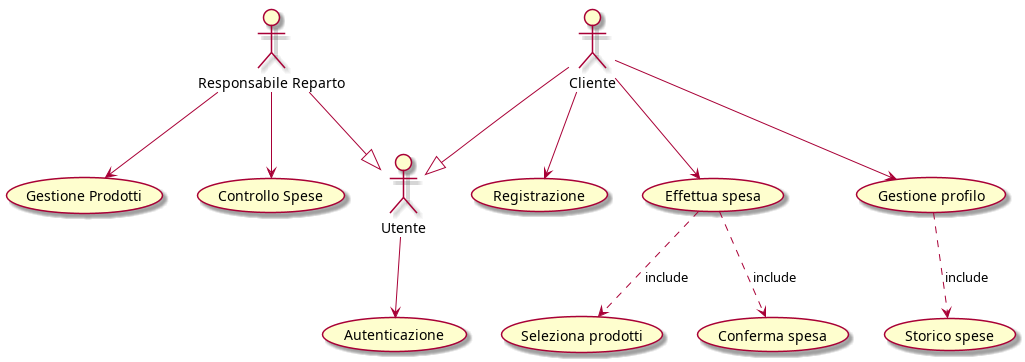
\includegraphics[width=\linewidth]{use_case_diagram.png}
\caption{Use case diagram}
\end{figure}

I due attori Cliente e Responsabile Reparto sono generalizzati nel attore Utente
per tutti gli use case di autenticazione, in quanto andranno ad autenticarsi
nello stesso portale.  Gli use case possono essere raggruppati in base 
all'attore a cui appartengono. Le funzioni principali del responsabile reparto 
sono di gestire prodotti e lo stato delle spese; gli use case del cliente sono
di registrarsi alla piattaforma, effettuare spese e gestire il proprio profilo.
Per tutti gli use case diversi dalla autenticazione o registrazione, prendiamo
come presupposto che l'utente sia già autenticato.

\newpage

\subsection{User Use Cases}

Le seguenti sono gli use case del utente con i corrispettivi sequence diagrams.

\subsubsection{Autenticazione}

\begin{figure}[H]
\centering
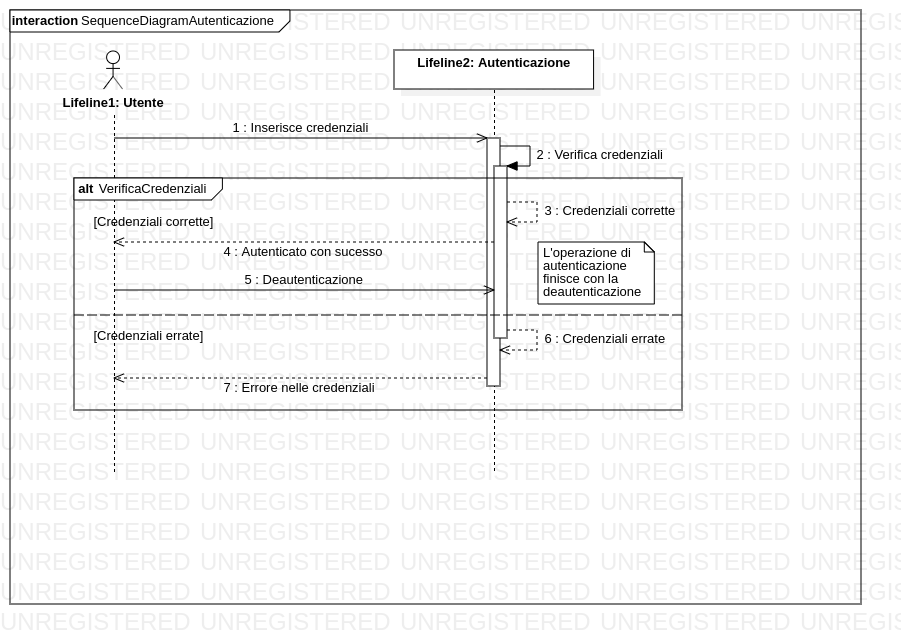
\includegraphics[width=\linewidth]{Use Case Model!Autenticazione!InteractionAutenticazione!SequenceDiagramAutenticazione_7.png}
\caption{Sequence diagram autenticazione}
\end{figure}

Quando l'utente deve autenticarsi, inserisce le credenziali nel portale. Queste
verranno verificate. Nel caso siano corrette verrà autenticato con successo, e 
potrà successivamente compiere il logout. Nel caso siano incorrette verrà
restituito un errore.

\newpage

\subsection{Responsabile Use Cases}

Le seguenti sono gli use case del responsabile del reparto con i corrispettivi 
sequence diagrams.

\subsubsection{Gestione Prodotti}

\begin{figure}[H]
\centering

\includegraphics[width=\linewidth]{Use Case Model!Gestione prodotti!InteractionGestioneProdotti!SequenceDiagramGestioneProdotto_9.png}
\caption{Sequence diagram gestione prodotti}
\end{figure}

Per la gestione dei prodotti il responsabile ha la possibilità di creare un nuovo
prodotto, modificarne o rimuoverne uno già esistente. La vista iniziale è una
lista dei prodotto, il responsabile può selezionarne uno e decidere se modificarlo
o rimuoverlo direttamente.

\subsubsection{Controllo Spese}

\begin{figure}[H]
\centering
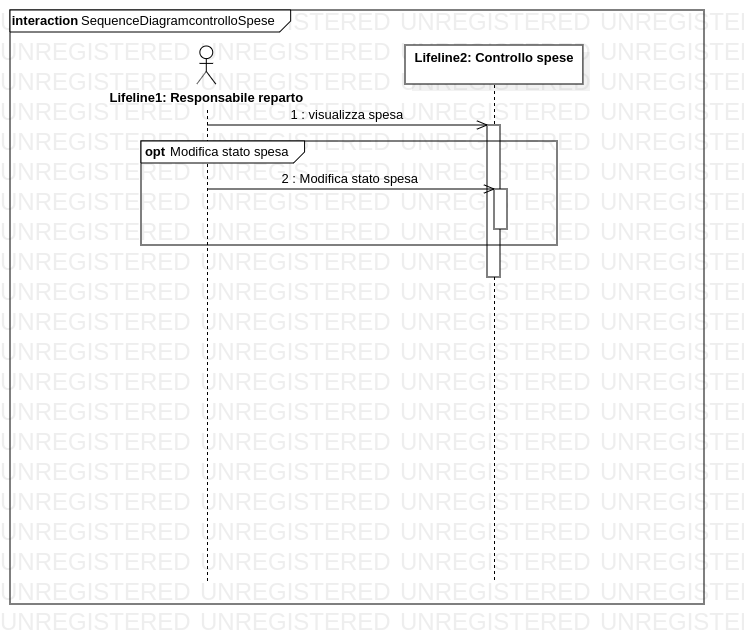
\includegraphics[width=\linewidth]{Use Case Model!Controllo spese!InteractionConstrolloSpese!SequenceDiagramcontrolloSpese_11.png}
\caption{Sequence diagram controllo spese}
\end{figure}

In fine per il controllo delle spese il responsabile ne visualizza una lista con
tutte le informazioni riguardanti ogni ordine e ha la possibilità di modificare
lo stato delle spese nella lista.

\newpage

\subsection{Client Use Cases}

Le seguenti sono gli use case del cliente con i corrispettivi sequence diagrams.

\subsubsection{Registrazione}

\begin{figure}[H]
\centering
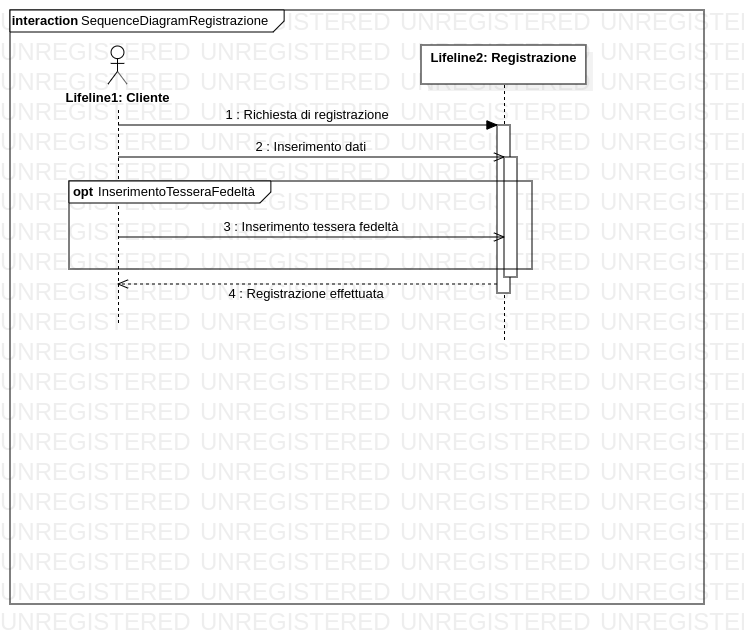
\includegraphics[width=\linewidth]{Use Case Model!Registrazione!InteractionRegistrazione!SequenceDiagramRegistrazione_1.png}
\caption{Sequence diagram registrazione}
\end{figure}

Il cliente accede alla vista della registrazione e dopo aver inserito i propri
dati ha la possibilità di inserire una tessera di fedeltà, facoltativa.

\subsubsection{Effettua Spesa}

\begin{figure}[H]
\centering
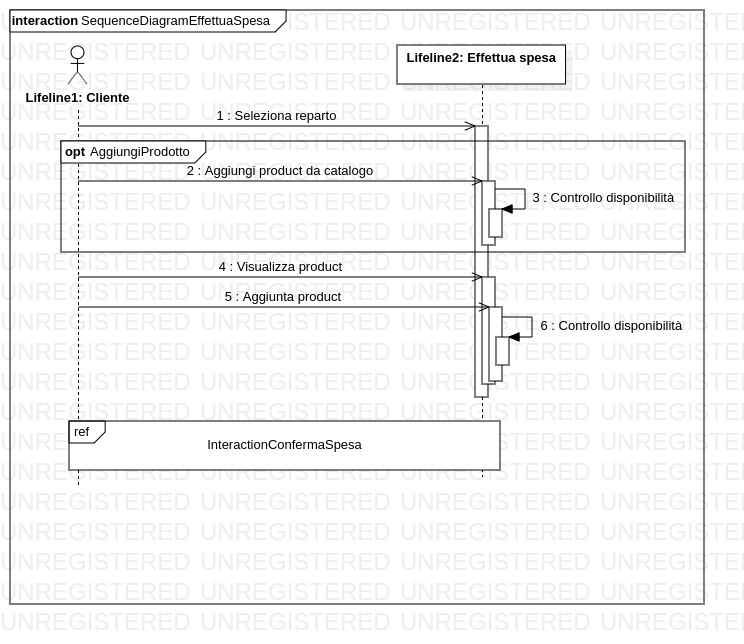
\includegraphics[width=\linewidth]{Use Case Model!Effettua spesa!InteractionEffettuaSpesa!SequenceDiagramEffettuaSpesa_3.png}
\caption{Sequence diagram effettua spesa}
\end{figure}


\begin{figure}[H]
\centering
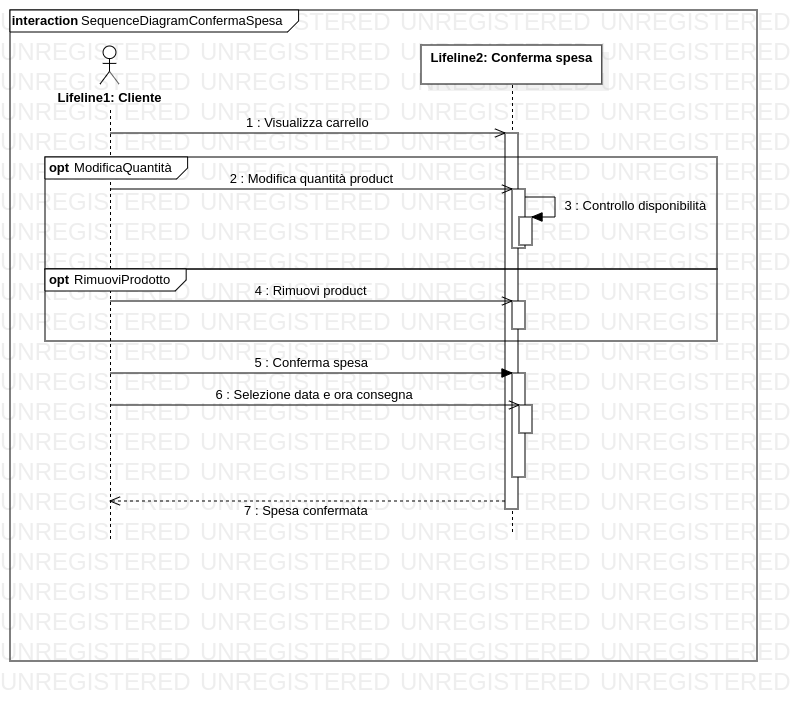
\includegraphics[width=\linewidth]{Use Case Model!Conferma spesa!InteractionConfermaSpesa!SequenceDiagramConfermaSpesa_13.png}
\caption{Sequence diagram effettua spesa}
\end{figure}

Per effettuare la spesa il cliente prima visualizza il catalogo dei prodotti. Qui
può selezionare le diverse categorie o cercare i prodotti che vuole aggiungere 
al carrello.

Quando ha aggiunto almeno un prodotto al carrello può visualizzarli e modificarne
la quantità o rimuoverli. Quando ha tutti i prodotto che gli servono può confermare
l'ordine e selezionare una data e un ora per la consegna.

\subsubsection{Gestione Profilo}

\begin{figure}[H]
\centering
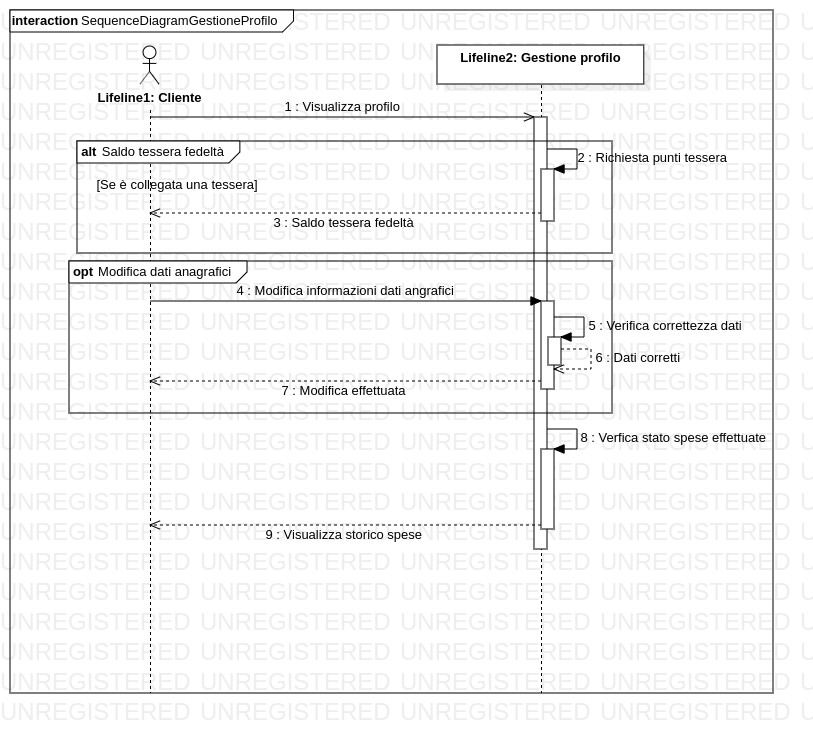
\includegraphics[width=\linewidth]{Use Case Model!Gestione profilo!InteractionGestioneProfilo!SequenceDiagramGestioneProfilo_5.png}
\caption{Sequence diagram gestione profilo}
\end{figure}

Nella gestione del profilo il cliente può vedere le proprie informazioni 
anagrafiche e modificarle. Inoltre se ha registrato una tessera fedeltà, sarà
possibile vedere il saldo dei punti guadagnati.

Dalla visualizzazione del profilo sarà possibile anche navigare alla
visualizzazione dello storico delle spese.

\newpage

\section{Activity diagram}

asd

% Activity diagram e spiegazione
\subsection{Autenticazione}
\begin{figure}[H]
\centering
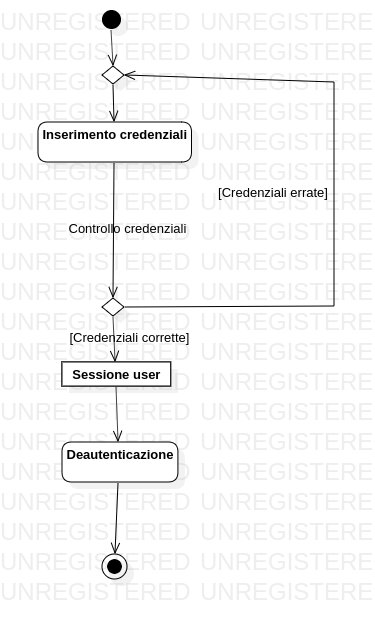
\includegraphics{Use Case Model!Autenticazione!ActivityAutenticazione!ActivityDiagramAutenticazione_8.png}
\caption{Activity diagram autenticazione}
\end{figure}

Il \textbf{cliente o il responsabile del reparto} inseriscono le credenziali username e password.
Il sistema le controlla e ritorna un messaggio di errore se queste sono scorrette, altrimenti crea una sessione che si occuperà della deautenticazione nel caso di Logout.

\emph{NOTA: Nell'implementazione finale è stato aggiunto un salvataggio della sessione, quindi con la chiusura dell'applicazione non si giungierà necessarriamente alla deautenticazione e quindi alla conclusione dell'Activity Diagram}.

\subsection{Conferma Spesa}
\begin{figure}[H]
\centering
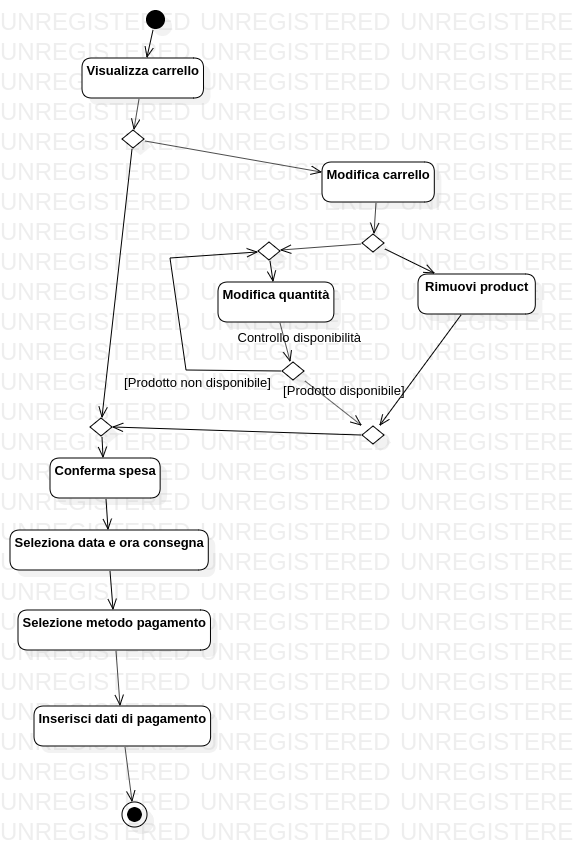
\includegraphics[width=\linewidth]{Use Case Model!Conferma spesa!ActivityConfermSpesa!ActivityDiagramConfermaSpesa_14.png}
\caption{Activity diagram Conferma Spesa}
\end{figure}

Il \textbf{cliente} registrato un Visualizza il proprio carrello. 
Una volta all'interno del carrello può Modificare le quantità, rimuovere il prodotto o confermare la spesa. 
Se modifica le quantità bisogna tener in considerazione la quantità di prodotti disponibili. 
Altrimenti se conferma bisognerà richiedere le informazioni per la consegna.
\emph{NOTA: Il metodo di pagamento viene ottenuto direttamente dalla session dell'utente}

\subsection{Visualizza Spesa}
\begin{figure}[H]
\centering
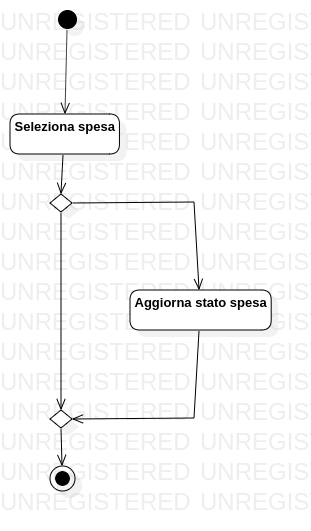
\includegraphics[width=\linewidth]{Use Case Model!Controllo spese!ActivityControlloSpese!ActivityDiagramControlloSpese_12.png}
\caption{Activity diagram Visualizza Spese}
\end{figure}

Il \textbf{responsabile di reparto} una volta autenticato e all'interno della visualizzazione della spesa, il responsabile può visualizzarne i prodotti di una spesa o aggiornarne lo stato.

\subsection{Effettua Spesa}
\begin{figure}[H]
\centering
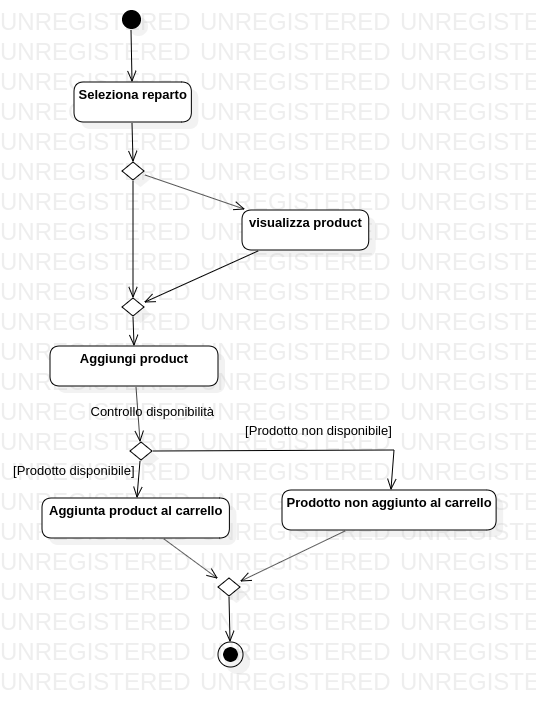
\includegraphics[width=\linewidth]{Use Case Model!Effettua spesa!ActivityeffettuaSpesa!ActivityDiagramEffettuaSpesa_4.png}
\caption{Activity diagram Effettua Spesa}
\end{figure}

Il \textbf{cliente} una volta autenticato e all'interno del catalogo potrà selezionare un reparto (di default preselezionato su All, contente tutti i prodotti a catalogo) e potrà aggiungiere prodotti al carrello sia dalla lista del catalogo direttamente sia cliccando sul item corrispondente e aggiungiendolo al carrello una volta aperta la scheda del prodotto corrispondente.
Prima dell'aggiunta il sistema controlla la disponibilità del prodotto e se è disponibile lo aggiungie al carrello.


\subsection{Modifica/Aggiungi Prodotto}
\begin{figure}[H]
\centering
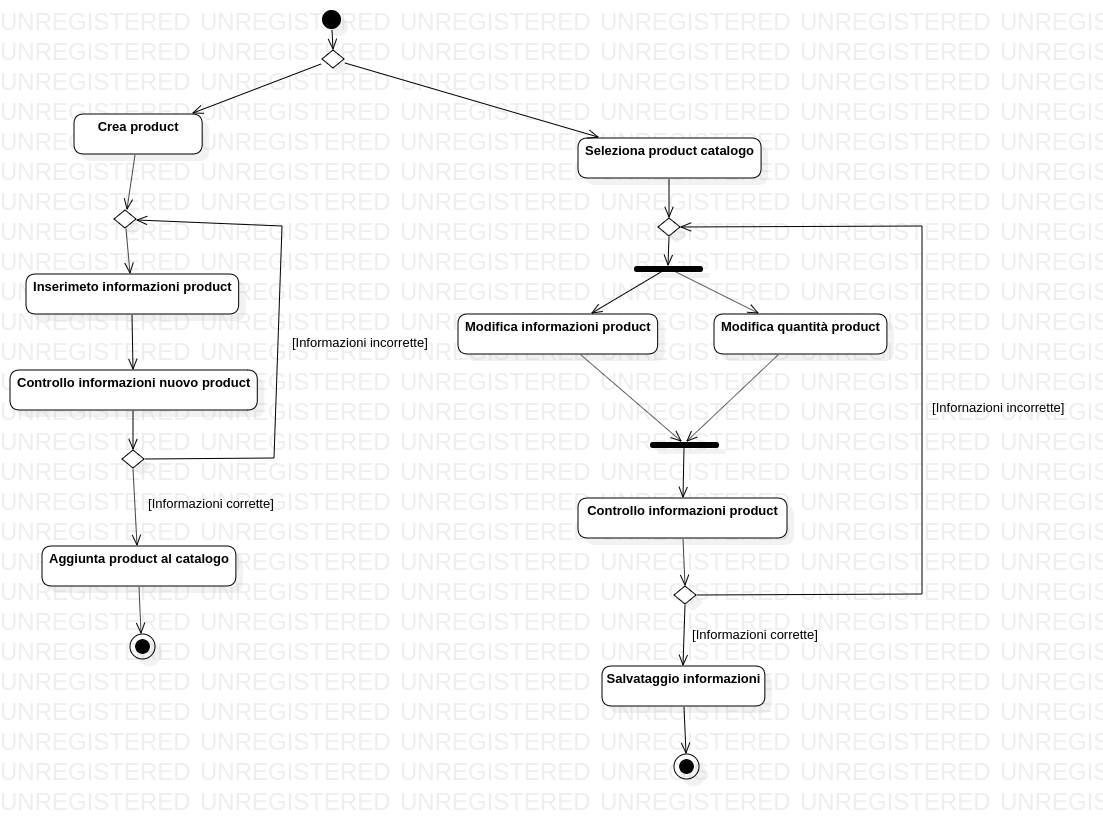
\includegraphics[width=\linewidth]{Use Case Model!Gestione prodotti!ActivityGestioneProdotti!ActivityDiagramGestioneProdotti_10.png}
\caption{Activity diagram Modifica o Aggiungi}
\end{figure}

Il \textbf{responsabile del reparto } una volta autenticato ed entrato nella gestione dei prodotti potrà decidere se creare un nuovo prodotto o selezionarne uno da catalogo per procedere alla modifica o alla rimozione.
Nel caso di creazione del prodotto inserisce le informazioni del prodotto che vengono controllate dal sistema prima dell'aggiunta nel catalogo.
Nel caso di modifica della quantità o modifica del prodotto sarà possibile selezionare il prodotto dalla lista. Una volta superati i controlli del sistema il prodotto  verrà aggiornato con le nuove informazioni.
\emph{NOTA: Nell'implementazione è stata aggiunta la à di rimuovere il prodotto selezionandolo dalla lista}


\subsection{Gestione Profilo}
\begin{figure}[H]
\centering
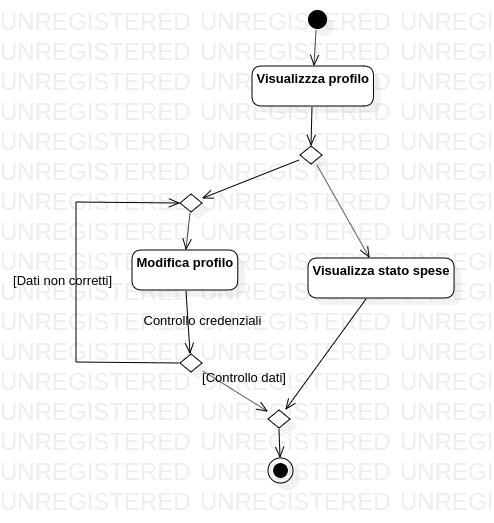
\includegraphics[width=\linewidth]{Use Case Model!Gestione profilo!Activity1!ActivityDiagramRegistrazione_6.png}
\caption{Activity diagram Visualizza Prodotto}
\end{figure}

Il \textbf{cliente} una volta autenticato e aver acceduto al proprio profilo può mdoifcare i propri dati o visualizzare lo stato delle proprie spese.
Nel caso di modifica dei dati il sistema provvederà alla verifica dei dati inseriti. Se i dati risultano corretti allora i salva.


\subsection{Registrazione}
\begin{figure}[H]
\centering
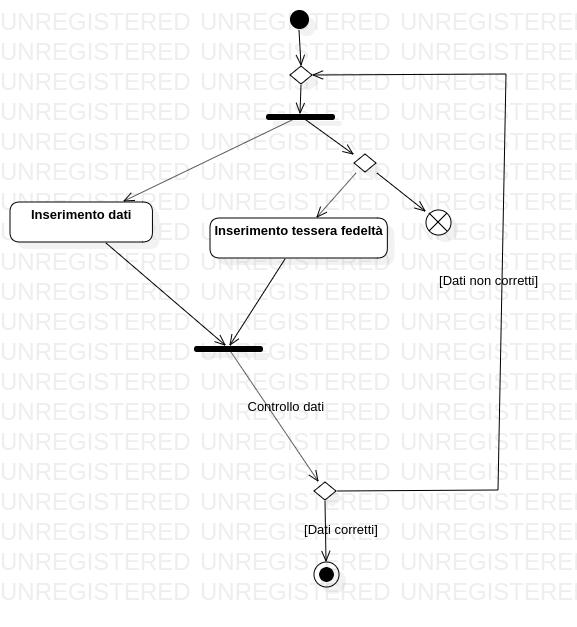
\includegraphics[width=\linewidth]{Use Case Model!Registrazione!ActivityRegistrazione!ActivityDiagramRegistrazione_2.png}
\caption{Activity diagram Registrazione}
\end{figure}

Il \textbf{cliente} prima di autenticarsi entra in registrazione ed inserisce i propri dati e se vuole la propria tessera fedeltà. 
Quindi il sistema verifica i dati inseriti, se sono corretti registra il nuovo utente altrimenti segnala un errore nella compilazione dei campi.

\section{Pattern architetturali}

asdfasd
% MVC Server Repository(Database)

\section{Class diagram}

Le classi nel sistema rispecchiano il pattern architetturale. Possiamo
considerarle come due sistemi diversi del client e il server. 

Nel server ci sono due classi principali il Router, per la gestione delle richieste
e il Database, che controlla i modelli. Questi ultimi nel client sono i model del
MVC, mentre i controllers gestiscono l'esecuzione dell'applicazione. Non tutti i campi
dei model nel Database sono presenti anche sul client, visto che sono utilizzati
per facilitare il funzionamento del database e non contengono vere informazioni.

Sia il server che il client contengono una classe Utils con solo metodi statici
che è stata crata per semplificare dei metodi e rende più modulare il codice.

% Riassunto enf. classi più importanti
% Mod nel database simi modl client non ug

\subsection{Server e Database}

Il Router ha il compito di gestire le chiamate del client e utilizza il database
e le classi dei model per ricavare le informazioni 

\begin{figure}[H]
\centering
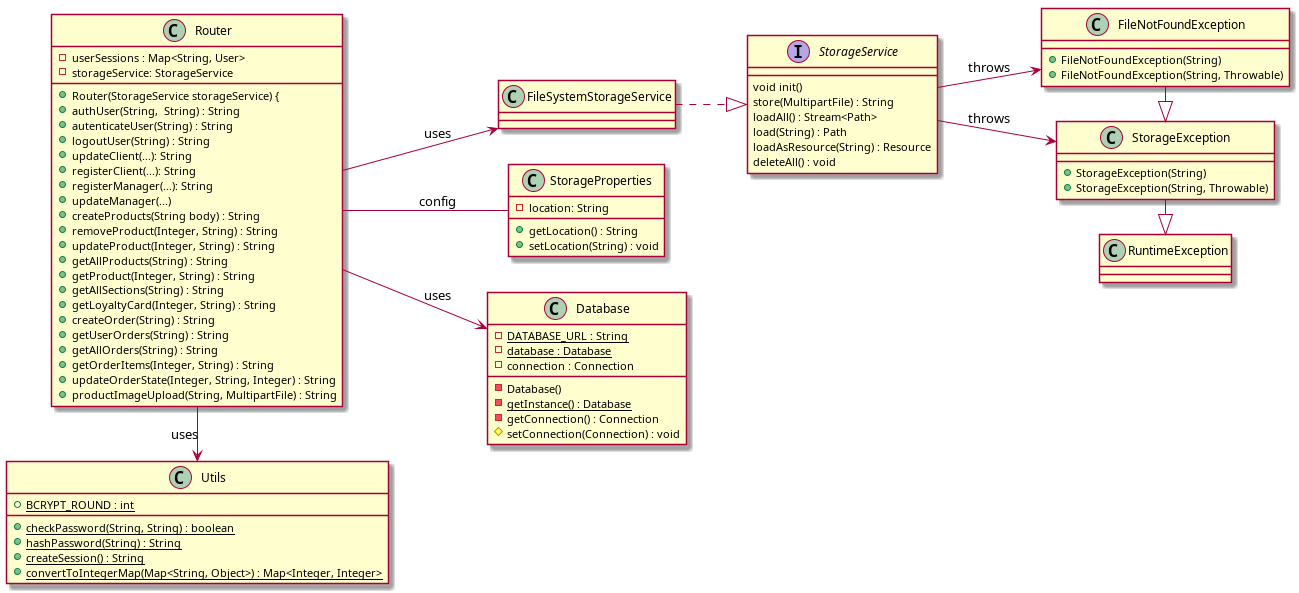
\includegraphics[width=\linewidth]{router_class.png}
\caption{Class diagram server}
\end{figure}

In aggiunta al database viene anche utilizzato lo FilesystemStorageService per
salvare le immagini dei prodotti caricate dagli utenti.

\subsection{Models}

Il database utilizza la classe Database per prendere una connessione al database
fisico e i diversi models per ricavare le informazioni.

\begin{figure}[H]
\centering
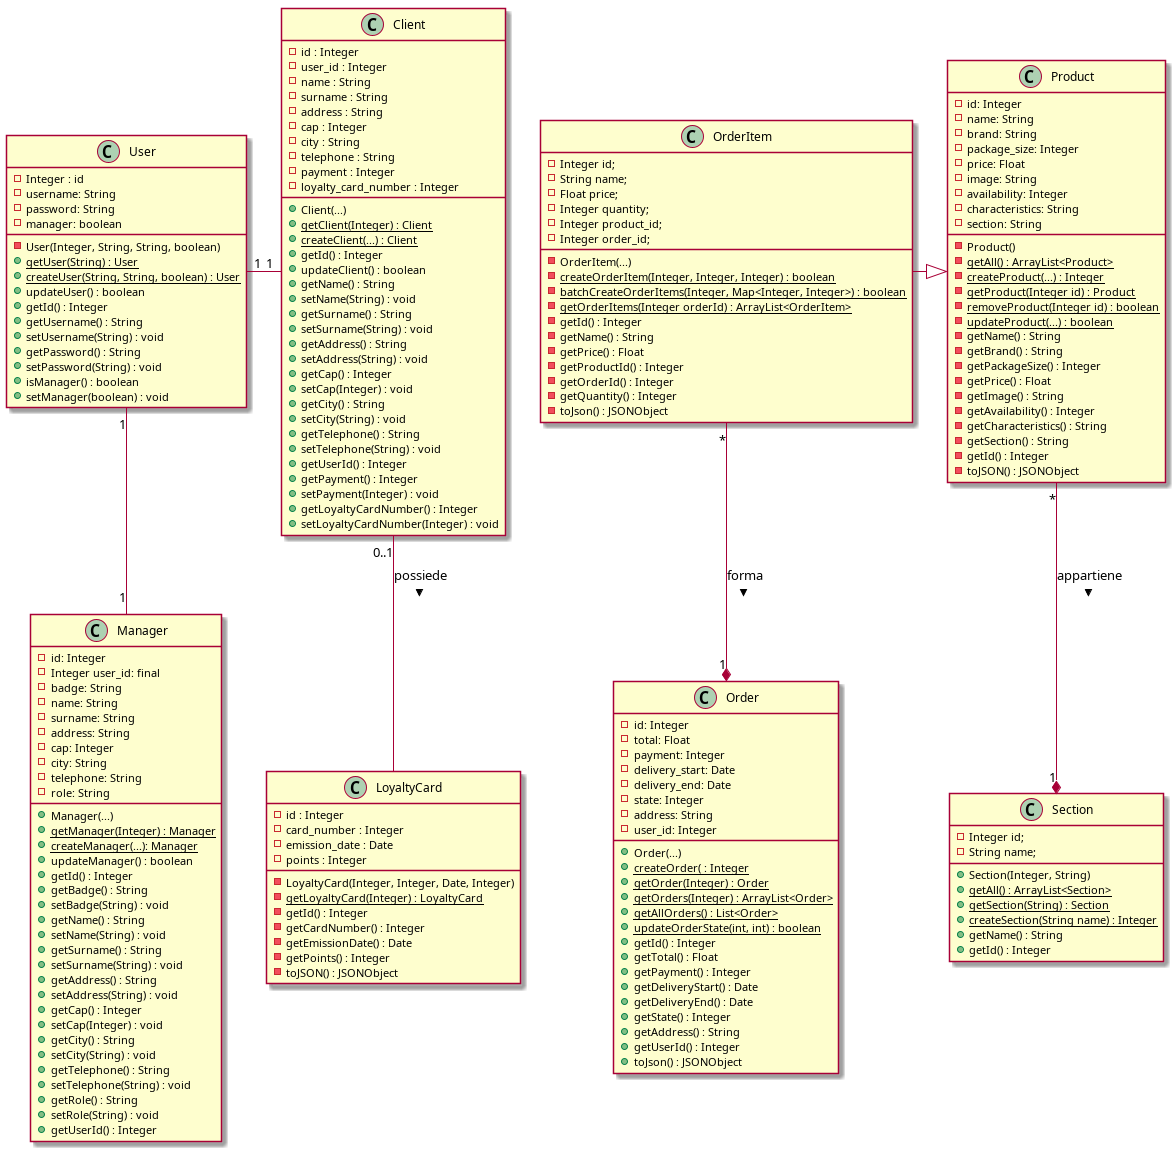
\includegraphics[width=\linewidth]{database_models_class.png}
\caption{Class diagram database}
\end{figure}

Invece nel client la Section non è più necessaria e non dovendo più rispettare lo
schema del database possiamo creare una generalizzazione del User, Client e Manager.

\begin{figure}[H]
\centering
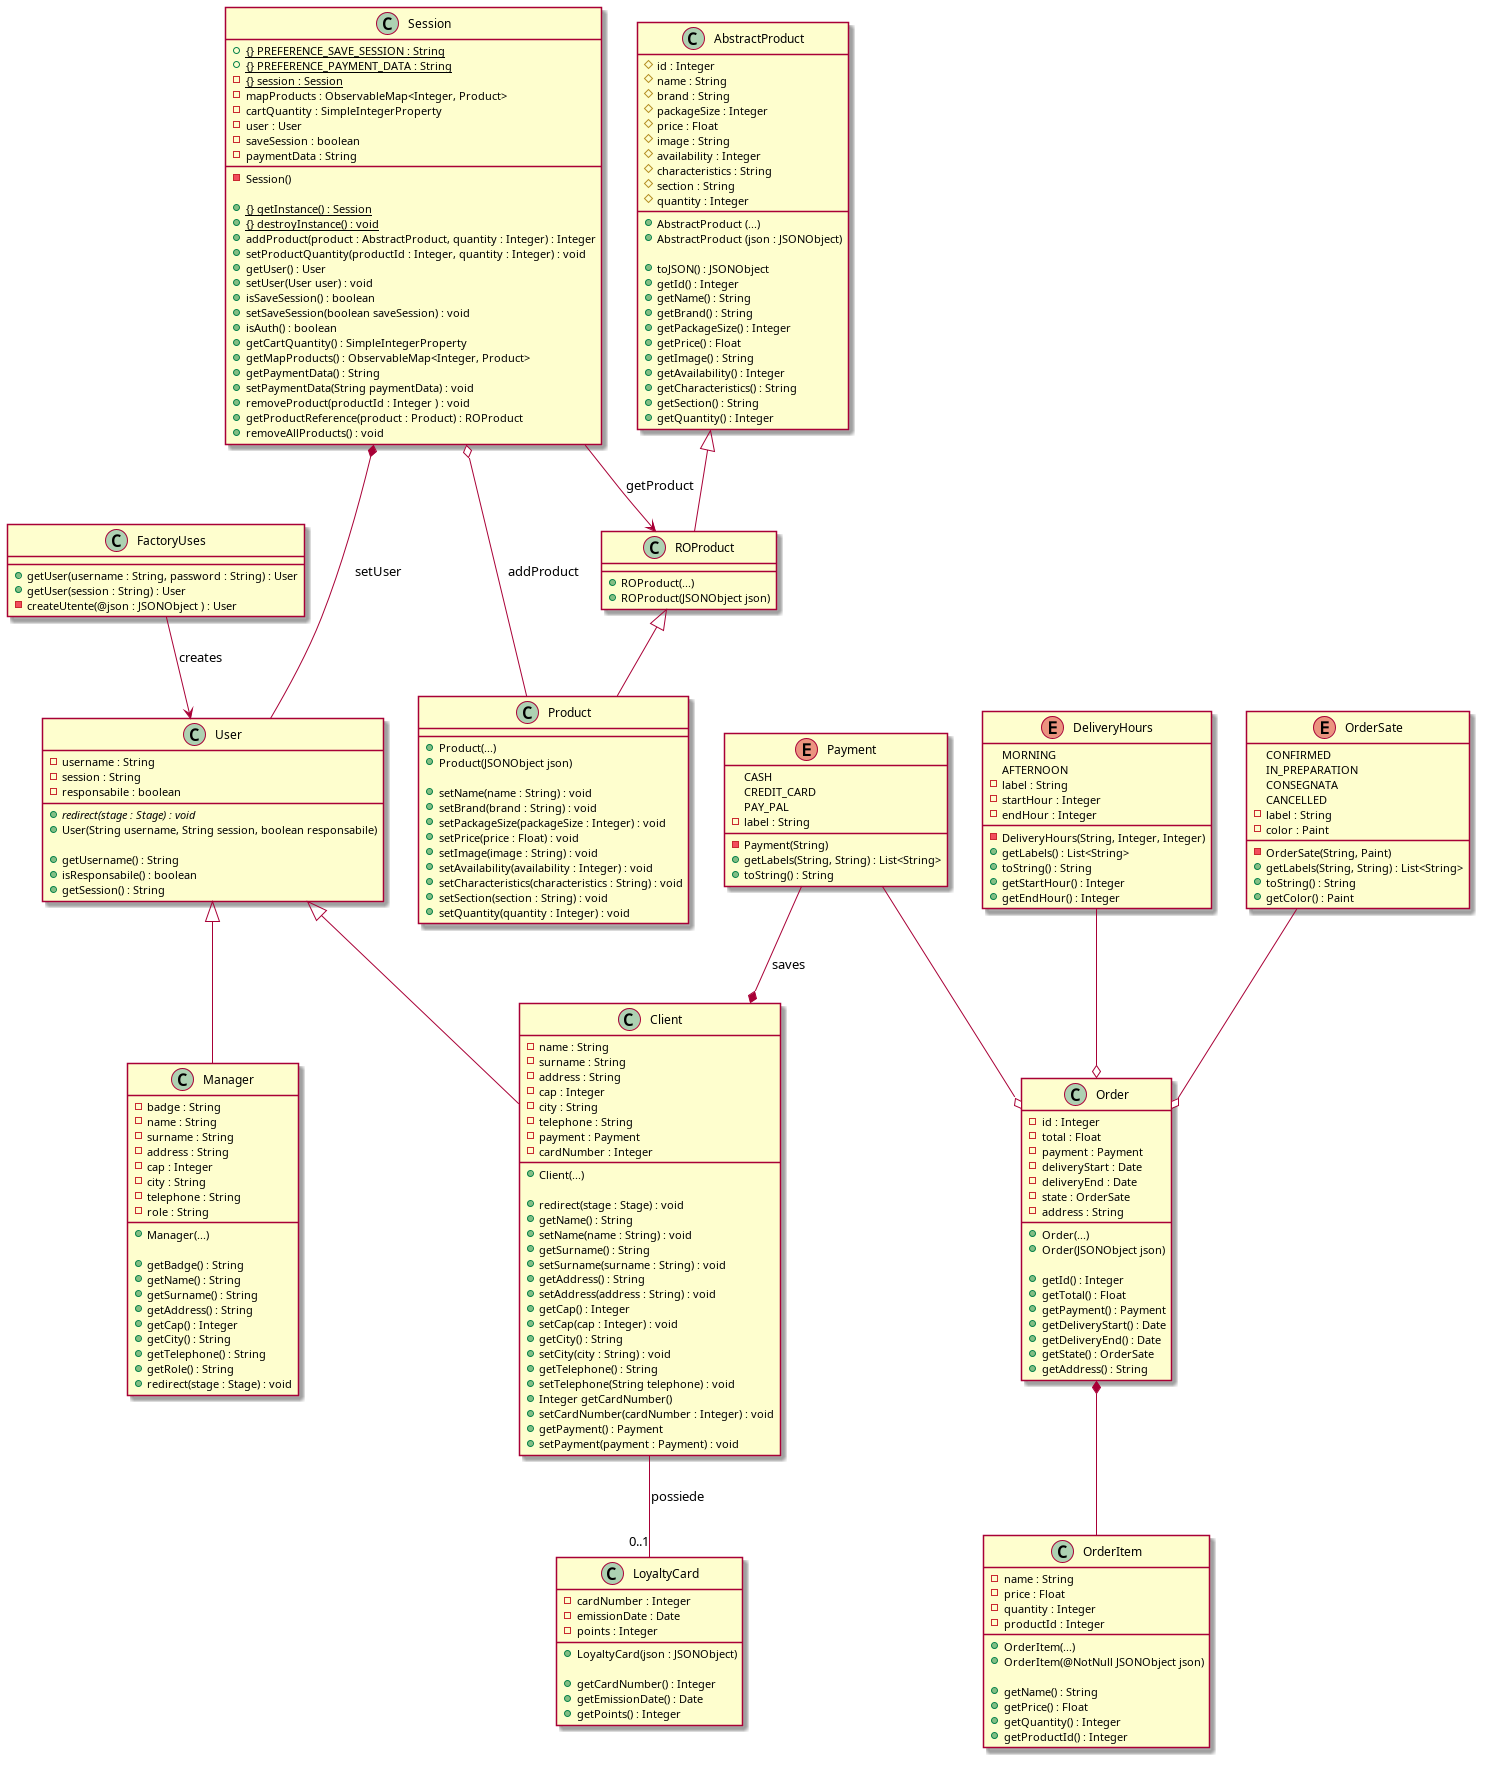
\includegraphics[width=\linewidth]{client_models_class.png}
\caption{Class diagram client models}
\end{figure}

% Classe della Sessione
%   con eventuali robe

\subsection{Controllers}

% Tasks & Components

\section{Discussione design patterns}

pppattern

% Singletons
%   Database
%   Sessione
% DAO Observable Sessione
% Factory
%   Utente
% Gli altri non sono factory, ma li abbiamo tenuti cosi per divisione del codice
% e possibile ottimizzazione

\section{Test suite}

Unit test

% TDD crea test, crea funzione intellij genera metodi
% Unit test tutto server, code coverage
% Javafx non testabile, ma funzioni attorno si
% CI/CD GitHub test automatici

\section{Conclusione}
Il progetto è stato condotto cercando inizialmente di rispettare le metodologia \textbf{Scrum} e utilizzando un \textbf{System Version Control} quale GIT per poter gestire al meglio il lavoro a distanza sullo stesso progetto. Dopo aver concordato degli sprint molto ristretti (una settimana circa) e avendo un brief ogni due giorni invece che 1, abbiamo cominciato col progetto.

\end{document}
